\chapter{Лекция 1 — 10 февраля 2025}

\section{Методологии}

\begin{listbox}{\noindent \begin{listboxtitle}{}5\end{listboxtitle}}
    \begin{enumerate}
		\item императивная — пошаговая работа ПК;
		\item функциональное;
		\item логическое;
		\item ООП;
		\item параллельное.
	\end{enumerate}
\end{listbox}

\section{Коротко о Lisp}

\begin{listbox}{\noindent \begin{listboxtitle}{}4\end{listboxtitle}}
\begin{enumerate}
	\item Идея Lisp(List Processing — обработчик списков) — математика + фунции, символьная обработка информации;
	\item аппрективный язык;
	\item безтиповый язык;
	\item нет синтаксической разницы между данными и программой.
\end{enumerate}
\end{listbox}

\section{Функциональное программирование}
Функциональное программирование определяет процессы вычисления на основе достаточно строгих 
абстрактных понятий и методов символьной обработки данных, а значит допускает высокий уровень
абстракции, позволяя выполнить формализацию множества объектов и определить полную семантическую
систему операций над объектами. 

При этом классы задач и их решений могут быть представлены строгими формулами. Формулы могут быть 
упрощены введением новых функциональных символов(данных, действий, формул), то есть система может быть 
консервативно расширена.

\textbf{Базис} — минимальный набор обозначений, к которым можно свести все правильные вычислительные формулы системы,
реализация которого является минимальной версией системы. Разные расширения базиса могут восприниматься 
как разные системы.

\begin{listbox}{\noindent \begin{listboxtitle}{}4\end{listboxtitle} 
	\raisebox{6pt}{Базис Lisp образуют:}}
\begin{enumerate}
	\item атомы;
	\item точечные пары;
	\item базовые функции;
	\item базовые функционалы.
\end{enumerate}
\end{listbox}

Системы, в которых можно включать любые символы, наделяя их смыслом, называются аппрекативными.

Разработка системы включает фазу формирования базиса и наполнение ядра системы в терминах, которые
не сводятся к её языку.

\section{S-выражения, атом, точечная пара}

Lisp использует S-выражения(символьные).

\begin{center}
	S-выражение ::= <атом>|<точечная пара>
\end{center}

\textbf{Атом} — неделимая последовательность символов.

\begin{listbox}{\noindent \begin{listboxtitle}{}3\end{listboxtitle} 
	\raisebox{6pt}{Атомы делятся на:}}
\begin{enumerate}
	\item символы(идентификаторы);
	\item специальные символы(T, Nil);
	\item самоопределимые атомы — числа, строки.
\end{enumerate}
\end{listbox}

\textbf{S-выражения} — все виды атомов + списки.

Более сложно организованные данные — списки и точечные пары, в памяти 
строятся из унифицированных структур — бинарных узлов.

\begin{center}
	<Точечная пара(тп)> ::= (<атом>.<атом>) || (<тп>.<атом>) || (<атом>.<тп>) || (<тп>.<тп>)
\end{center}

<Список> ::= <пустой список> | <непустой список>, где:

\begin{itemize}[label=—]
	\item <пустой список> ::= () | Nil;
	\item <непустой список> ::= (<первый элемент>.<хвост>);
	\item <первый элемент> ::= <S-выражение>;
	\item <хвост> ::= <список>.
\end{itemize}

\begin{figure}[H]
    \begin{imagebox}
        \centering
        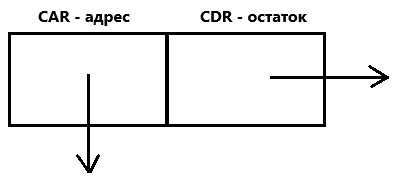
\includegraphics[width=0.8\textwidth]{img/car-cdr.png}
        \label{fig:tp-car-cdr}
    \end{imagebox}
    \caption{Расположение точечной пары в памяти.}
\end{figure}

Функции car/cdr — переход по car/cdr указателю.

\section{Структуры}

() — признак структуры.

Список (A B C), где A — имя функции.

Пример: (car '(A B C))